%!TEX root = ../../super_main.tex

\section{Continuous Integration}
\label{sec:continuous_integration}
As mentioned in \secref{sec:extreme_programming}, we wanted a Continuous Integration (CI) server in order to help us keep our code base stable. We installed Jenkins on the same server that makes up the server part of our client-server architecture, because it was easily available. Jenkins is an open source automation server, which supports various different plugins that helps with automated builds, running tests and showing the results of those, etc. We configured the Jenkins server to be notified whenever any changes were made to the master branch of our Android or PHP Git repositories (hosted on GitHub). When notified, Jenkins will build the corresponding project and automatically run its test suite. Whenever a project would go from a previously successful build to a failing build or vice versa, the Jenkins system would send out mails to our group, notifying us that something went wrong or that it was back to normal. If a build failed, the mail would contain information regarding which tests failed, and their stack trace. This made it possible for us to give immediate attention to issues that we did not catch before pushing our content to the version control. \figref{fig:jenkins_front_page} shows the front page of the Jenkins website. In the left side, the build queue is seen, which shows if any builds are currently running. Jenkins displays helpful information about the state of the configured projects. The blue circle, depicted in the figure, changes to red if the most recent build was a failure, and besides that, it is how long time has passed since the most recent pass, most recent failure, and how long the last build took to finish. By clicking on one of the projects, different code and quality metrics will be shown, such as checkstyle warnings, code coverage, and test results. 

\begin{figure}[!htbp]
    \centering
    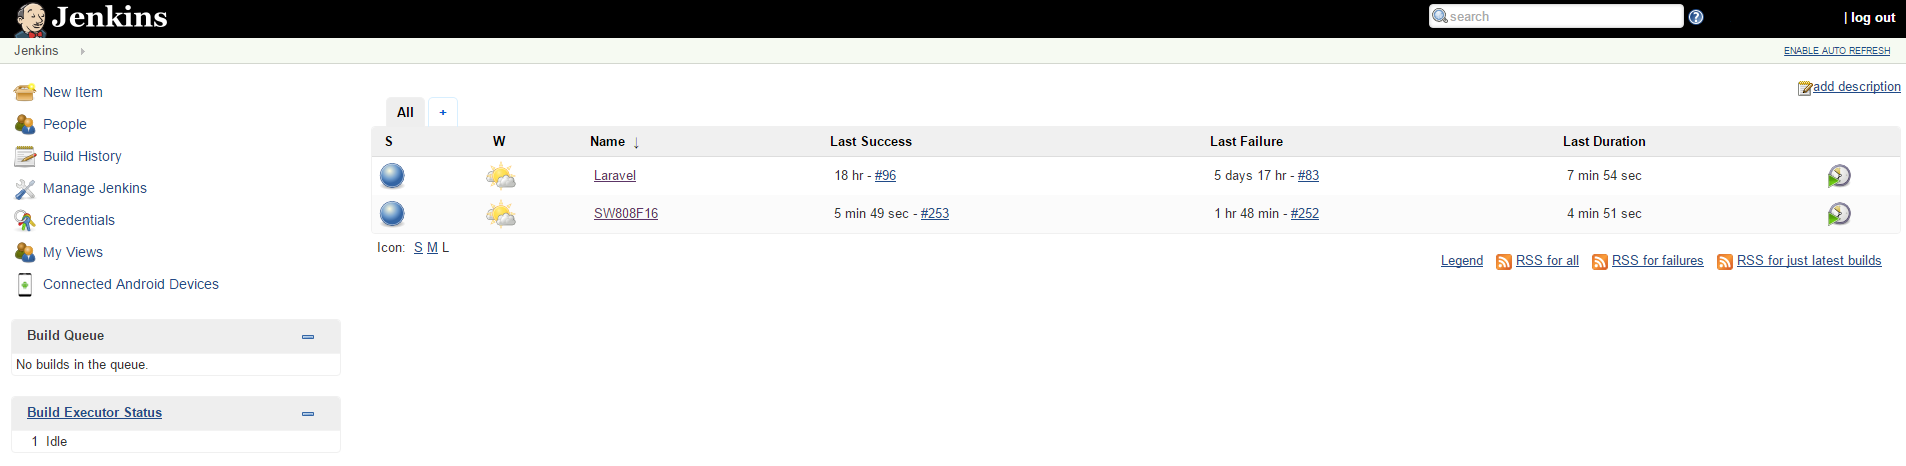
\includegraphics[width=\textwidth]{graphic/quality_assurance/jenkins_frontpage}
    \caption{Jenkins CI front page.}
    \label{fig:jenkins_front_page}
\end{figure}
\FloatBarrier

In our development we have utilized feature branching \parencite{feature_branching}, where each new feature would be developed on its own branch, and then, when finished, merged with the master branch. The master branch should for this reason never contain incomplete features. Previous experience with this work flow have shown that the process of merging with the master branch is error prone. Jenkins helped us unveil these errors, and ensured that we always knew if any of our tests failed, making us able to allocate people for fixing it. 
